%%%%%%%%%%%%%%%%%%%%
\newcommand{\functionANHTAO}[2]{
	\functionSignature{\texttt{anhtao-path}}{\varAtomicTask{}{}, \varAgent{}{}}
}

\subsection{Algorithm for optimising hierarchical task allocation in networks of agents}

The \acronymWSNOptimisationExtended{}{} algorithm is defined in Algorithms \ref{alg:wsn_optimisation_sink}
and \ref{alg:wsn_optimisation_arc}, which are split for clarity. The flowchart in Figure \ref{fig:algorithm-flow} shows how agents in the system allocate atomic tasks, and choose actions, as part of a composite tasks' execution.

\begin{figure}[ht]
	\centering
	\begin{subfigure}{.49\textwidth}
		\centering
		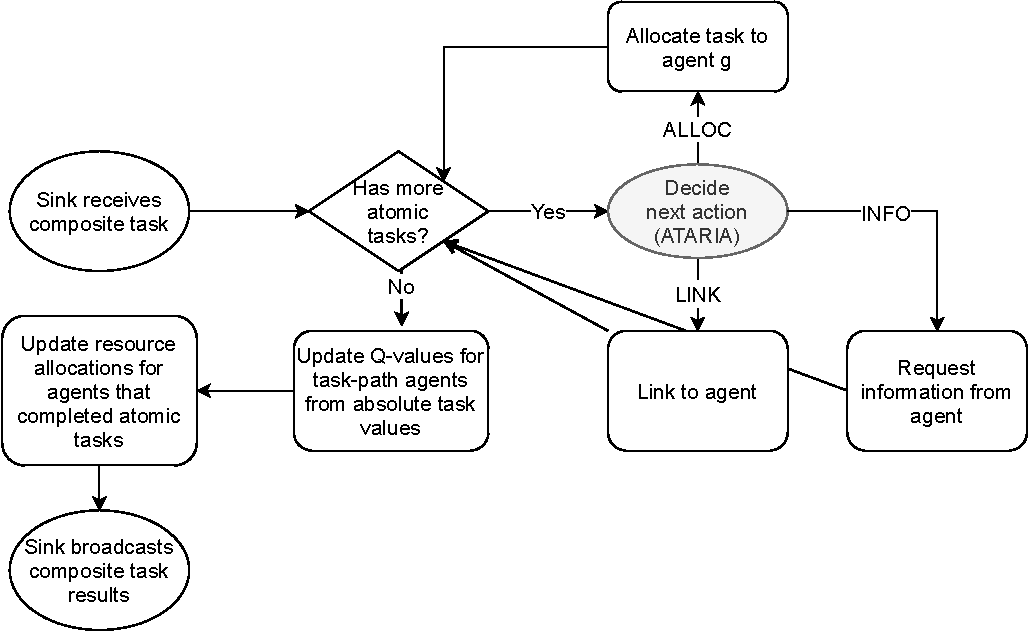
\includegraphics[width=0.9\linewidth, trim={25pt 0pt 25pt 0pt, clip}]{algorithm-flow-sink}
		\caption{Sink agent flow}
		\label{fig:algorithm-flow-sink}
	\end{subfigure} \hfill%
	\begin{subfigure}{.49\textwidth}
		\centering	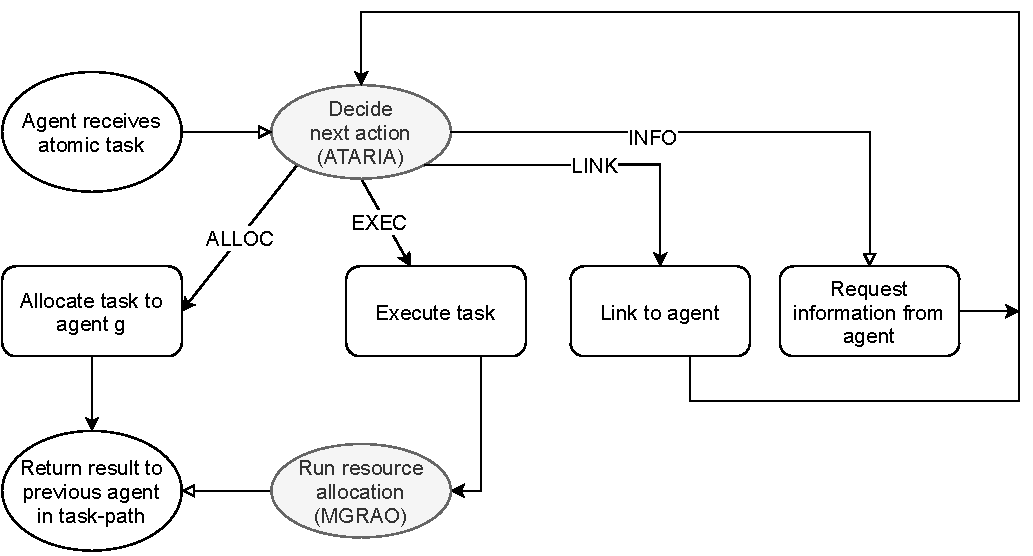
\includegraphics[width=0.9\linewidth,trim={25pt 0pt 25pt 0pt, clip}]{algorithm-flow-arc}
		\caption{Task-path agent flow}
		\label{fig:algorithm-flow-arc}
	\end{subfigure}
	\caption{\textbf{\acronymWSNOptimisation{}{}} - Flow chart of combined \acronymATARIA{}{}/\acronymMGRAO{}{} execution. The two algorithms are combined together to allow recursive allocation of tasks and learning of the network.}
	\label{fig:algorithm-flow}
\end{figure}
We formally define the \acronymWSNOptimisation{}{} algorithm in two parts, Algorithm \ref{alg:wsn_optimisation_sink} for sink agents receiving composite tasks, and Algorithm \ref{alg:wsn_optimisation_arc} for other agents that form the task-path for a task.

In the \acronymWSNOptimisationSink{}{} algorithm, Algorithm \ref{alg:wsn_optimisation_sink}, the sink agent receives a composite task $\varCompositeTask{}{}$ comprising of multiple atomic tasks $\varAtomicTask{}{}$ to be completed. For each of these atomic tasks the sink agent runs the \acronymATARIA{}{} algorithm to select an action (Line \ref{wsnsink:select}). It can execute the atomic task itself (Line \ref{wsnsink:exec}), using the \acronymMGRAO{}{} algorithm to determine the resources that will be allocated to its completion,   m or allocate it to another agent it knows about to complete using the \acronymWSNOptimisationArc{}{} algorithm (Line \ref{wsnsink:alloc}) . In both cases, the sink agent receives an atomic task quality value of $\functionAtomicTaskQualitySignature{}{}$ and removes the atomic task from the list of tasks to complete. If the action selected is one of $\functionInfo{}{}$ or $\functionLink{}{}$, those actions are carried out without any task executions. Once all atomic tasks have completed, each atomic tasks' proportional value to the composite task is calculated. For each atomic task, the corresponding value is sent to the last agent in the atomic tasks' task-path so that each sensor agent can carry out an \acronymMGRAO{}{}-update to re-allocate its resources to increase the tasks' value in the future (Lines \ref{wsnsink:arc_last} and \ref{wsnsink:mgrao}). 

\newcommand{\nosemic}{\renewcommand{\@endalgocfline}{\relax}}% Drop semi-colon ;
\newcommand{\dosemic}{\renewcommand{\@endalgocfline}{\algocf@endline}}% Reinstate semi-colon ;
\newcommand{\pushline}{\Indp}% Indent
\newcommand{\popline}{\Indm\dosemic}% Undent
\let\oldnl\nl% Store \nl in \oldnl
\newcommand{\nonl}{\renewcommand{\nl}{\let\nl\oldnl}}% Remove line number for one line
\begin{algorithm}[ht]
	\DontPrintSemicolon
	\footnotesize
	
	\caption{\textbf{The \acronymWSNOptimisationSink{}{} algorithm}}
	\label{alg:wsn_optimisation_sink}
	{
		\KwIn{ $\varCompositeTask{}{}$ , The composite task set}
		\KwIn{ $\varAgent{self}{}$ , The sink agent completing the composite task}
		\KwResult{$\functionCompositeTaskQuality{}{}{}{}$ , The composite task quality of $\varCompositeTask{}{}$}		\nonl \;
		\tcp{Copy set of atomic tasks to list of incomplete tasks}
		$ctactive \leftarrow \varCompositeTask{}{}$ \label{wsnsink:copy}\;
		\For{$\varAtomicTask{}{} \in ctactive$\label{wsnsink:composite_tasks}}
		{
			\tcp{Select action through \acronymATARIA{}{}}
			$\varAction{}{} \leftarrow \functionATARIA{}{}$ \label{wsnsink:select} \;	
			\uIf{$\varAction{}{} = \functionExec{}{}$?}
			{
				\tcp{Execute task $\varAtomicTask{}{}$ and get an atomic task quality} 
				$\functionAtomicTaskQualitySignature{}{} \leftarrow \functionExec{}{}$ \label{wsnsink:exec}\;
				\tcp{Remove atomic task from incomplete task list}
				$ctactive{}{} \leftarrow ctactive - \lbrace \varAtomicTask{}{} \rbrace$ \label{wsnsink:exec_remove}\;
			}
			\uElseIf{$\varAction{}{} = \functionAlloc{}{}$?}{
				\tcp{allocate task $\varAtomicTask{}{}$ to agent} $\functionAtomicTaskQualitySignature{}{} \leftarrow \functionANHTAO{}{}$\label{wsnsink:alloc} \;
				\tcp{Remove atomic task from incomplete task list}
				$ctactive{}{} \leftarrow ctactive{}{} - \lbrace \varAtomicTask{}{} \rbrace$ \label{wsnsink:alloc_remove}\;
			}
			\uElseIf{$\varAction{}{} = \functionInfo{}{}$?}{
				\tcp{request information on system agents from agent $\varAgent{}{}$}
				$\functionInfo{}{}$ \label{wsnsink:info}\;
			}
			\uElseIf{$\varAction{}{} = \functionLink{}{}$?}{
				\tcp{allocate resources to information on to agent $\varAgent{}{}$ and maintaining network connection}
				$\functionLink{}{}$ \label{wsnsink:link}\;
			}
		}
		\For{$\varAtomicTask{}{} \in \varCompositeTask{}{}$\label{ataria:composite_tasks}}
		{
			\tcp{Target update at the last agent in the task-path, the agent that completed the atomic task}
			$\varAgent{}{} \leftarrow \functionSenseRole{}{}$ \label{wsnsink:arc_last}\;
			\tcp{Send the sensor agent the atomic task value to run the MGRAO update}
			$\functionMGRAOUpdate{}{}$ \label{wsnsink:mgrao}\;	
		}
		\Return{$\functionCompositeTaskQuality{}{}{}{}$}
	}
\end{algorithm}

The \acronymWSNOptimisationArc{}{} algorithm (Algorithm \ref{alg:wsn_optimisation_arc}) will complete an atomic task and return its quality, either by executing the task itself (Line \ref{wsnarc:exec}), or re-allocating to another agent (Line \ref{wsnarc:alloc}). The \acronymATARIA{}{} algorithm is run and an action selected (Line \ref{wsnarc:select}), in the same way as in the \acronymWSNOptimisationSink{}{} algorithm. The selection and execution of actions using the \acronymATARIA{}{} algorithm is repeated until the task in completed an atomic task quality can be returned (Line \ref{wsnarc:exec}).
\begin{algorithm}[ht]
	\DontPrintSemicolon
	\footnotesize
	
	\caption{\textbf{The \acronymWSNOptimisationArc{}{} algorithm } }
	\label{alg:wsn_optimisation_arc}
	{
		\KwIn{ $\varAtomicTask{}{}$ , The atomic task to be completed}
		\KwIn{ $\varAgent{self}{}$ , The agent completing the composite task}
		\KwResult{$\functionAtomicTaskQualitySignature{}{}$ , The atomic task quality of $\varAtomicTask{}{}$}
		\nonl \;
		
		$taskComplete \leftarrow False$ \;
		\While{$\neg taskComplete$ }{
		\tcp{Select action through \acronymATARIA{}{}}
		$\varAction{}{} \leftarrow \functionATARIA{}{}$ \label{wsnarc:select} \;	
		\uIf{$\varAction{}{} = \functionExec{}{}$?}
		{
			\tcp{Execute task $\varAtomicTask{}{}$ and get an atomic task quality} 
			$\functionAtomicTaskQualitySignature{}{} \leftarrow \functionExec{}{}$ \label{wsnarc:exec}\;
			$taskComplete \leftarrow True$ \;
		}
		\uElseIf{$\varAction{}{} = \functionAlloc{}{}$?}{
			\tcp{allocate task $\varAtomicTask{}{}$ to agent} $\functionAtomicTaskQualitySignature{}{} \leftarrow \functionANHTAO{}{}$\label{wsnarc:alloc} \;
			
			\tcp{allocate task $\varAtomicTask{}{}$ to agent $\varAgent{}{}$}
			$\functionAtomicTaskQualitySignature{}{} \leftarrow \functionAlloc{}{}$\label{wsnarc:alloc} \;
			$taskComplete \leftarrow True$ \;
			}
		\uElseIf{$\varAction{}{} = \functionInfo{}{}$?}{
			\tcp{request information on system agents from agent $\varAgent{}{}$}
			$\functionInfo{}{}$ \label{wsnarc:info}\;
		}
		\uElseIf{$\varAction{}{} = \functionLink{}{}$?}{
			\tcp{allocate resources to information on to agent $\varAgent{}{}$ and maintaining network connection}
			$\functionLink{}{}$ \label{wsnarc:link}\;
		}
	}
	\Return{$\functionAtomicTaskQualitySignature{}{}$\label{wsnarc:return}} \;
	}
\end{algorithm}
